\documentclass[handout]{beamer}
\usepackage{presentation}

\title{Сервис поиска электронных книг }
\subtitle{Серверная часть, обеспечивающая верификацию, обновление данных и взаимодействие с клиентскими программами и пользователем.}
%\author{Екатерина Тузова}
%\institute{АУ РАН}
\date{}


\begin{document}

\begin{frame}
  \titlepage
  \begin{flushright}
    Студент~~~~~~  Е. А. Тузова
  
    Руководитель~~~  Н. М. Пульцин

  \end{flushright}
\end{frame}

\section*{План презентации}
  \begin{frame}
    \frametitle{План презентации}
    \tableofcontents[pausesections]

  \end{frame}

\section{Описание проблемы}
  \begin{frame}

    \frametitle{Описание проблемы}
    \begin{enumerate}
      \item История (библиотеки, книжные магазины)
      \item Интернет (электронные библиотеки)
      \item Проблема поиска
      \item Проблема единого интерфейса
      \item Проблема многих форматов книг
      \end{enumerate}
  \end{frame}

\section{Обзор существующих решений}
  \begin{frame}
    \frametitle{Обзор существующих решений}

    \begin{enumerate}
      \item Google books
      \item Проект eBdb
      \item Amazon Kindle, Sony Reader
      \item OPDS
      \item BookServer
    \end{enumerate}
  \end{frame}

\section{Описание системы в целом}
  \begin{frame}
    \frametitle{Описание системы в целом}

    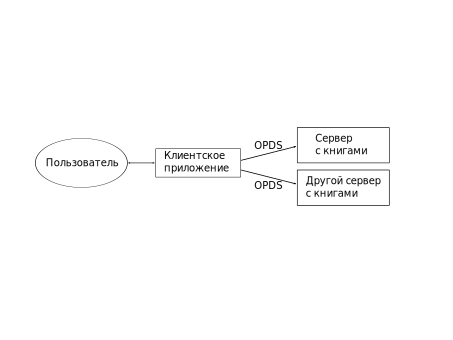
\includegraphics{./head/scheme}
  \end{frame}

\section{Задача обновления информации}
  \begin{frame}
    \frametitle{Задача обновления информации}
  
    \begin{enumerate}
      \item Определение жанра книги
      \item Поиск информации на внешних ресурсах
      \item Извлечение информации из форматов epub и fb2 
    \end{enumerate}
  \end{frame}

\section{Определение жанра книги}
  \begin{frame}
    \frametitle{Определение жанра книги}  
    
    \begin{enumerate}
      \item Возможные решения (плюсы и минусы)
      \item Байесов классификатор
    \end{enumerate}        
  \end{frame}

\subsection{Возможные решения}
  \begin{frame}
    \frametitle{Возможные решения}  
    
    \begin{enumerate}
      \item Деревья принятия решений
      \item Нейронные сети
      \item Метод k-средних
      \item Байесовский классификатор
    \end{enumerate}        
  \end{frame}


\section{Заключение}
  \begin{frame}
    \frametitle{Заключение}
  
  \end{frame}

\end{document}